\chapter{Exemplos}

\section{Un exemplo de sección}
Esta é {\it letra cursiva}, esta é {\bf letra negrilla}, esta é \underline{letra subrallada}, e esta é {\tt letra curier}. Letra {\tiny tiny}, {\scriptsize scriptsize}, {\small small}, {\large large}, {\Large Large}, {\LARGE LARGE} e moitas más. Exemplo de fórmula: $a=\int_o^\infty f(t)dt$.  E agora unha ecuación aparte:

\begin{equation}
S=\sum_{i=0}^{N-1} a_i^2 .
\label{mi_ecuacion}
\end{equation}

As ecuaciones se poden referenciar: ecuación (\ref{mi_ecuacion}).

\subsection{Un exemplo de subsección}
O texto vai aquí.
\subsection{Otro exemplo de subsección}
O texto vai aquí.
\subsubsection{Un exemplo de subsubsección}
O texto vai aquí.
\subsubsection{Un exemplo de subsubsección}
O texto vai aquí.
\subsubsection{Un exemplo de subsubsección}
O texto vai aquí.
\section{Exemplos de figuras e cadros}

A figura número \ref{enlace1}.

O cadro (taboa) número \ref{enlace2}.

\begin{figure}
\centerline{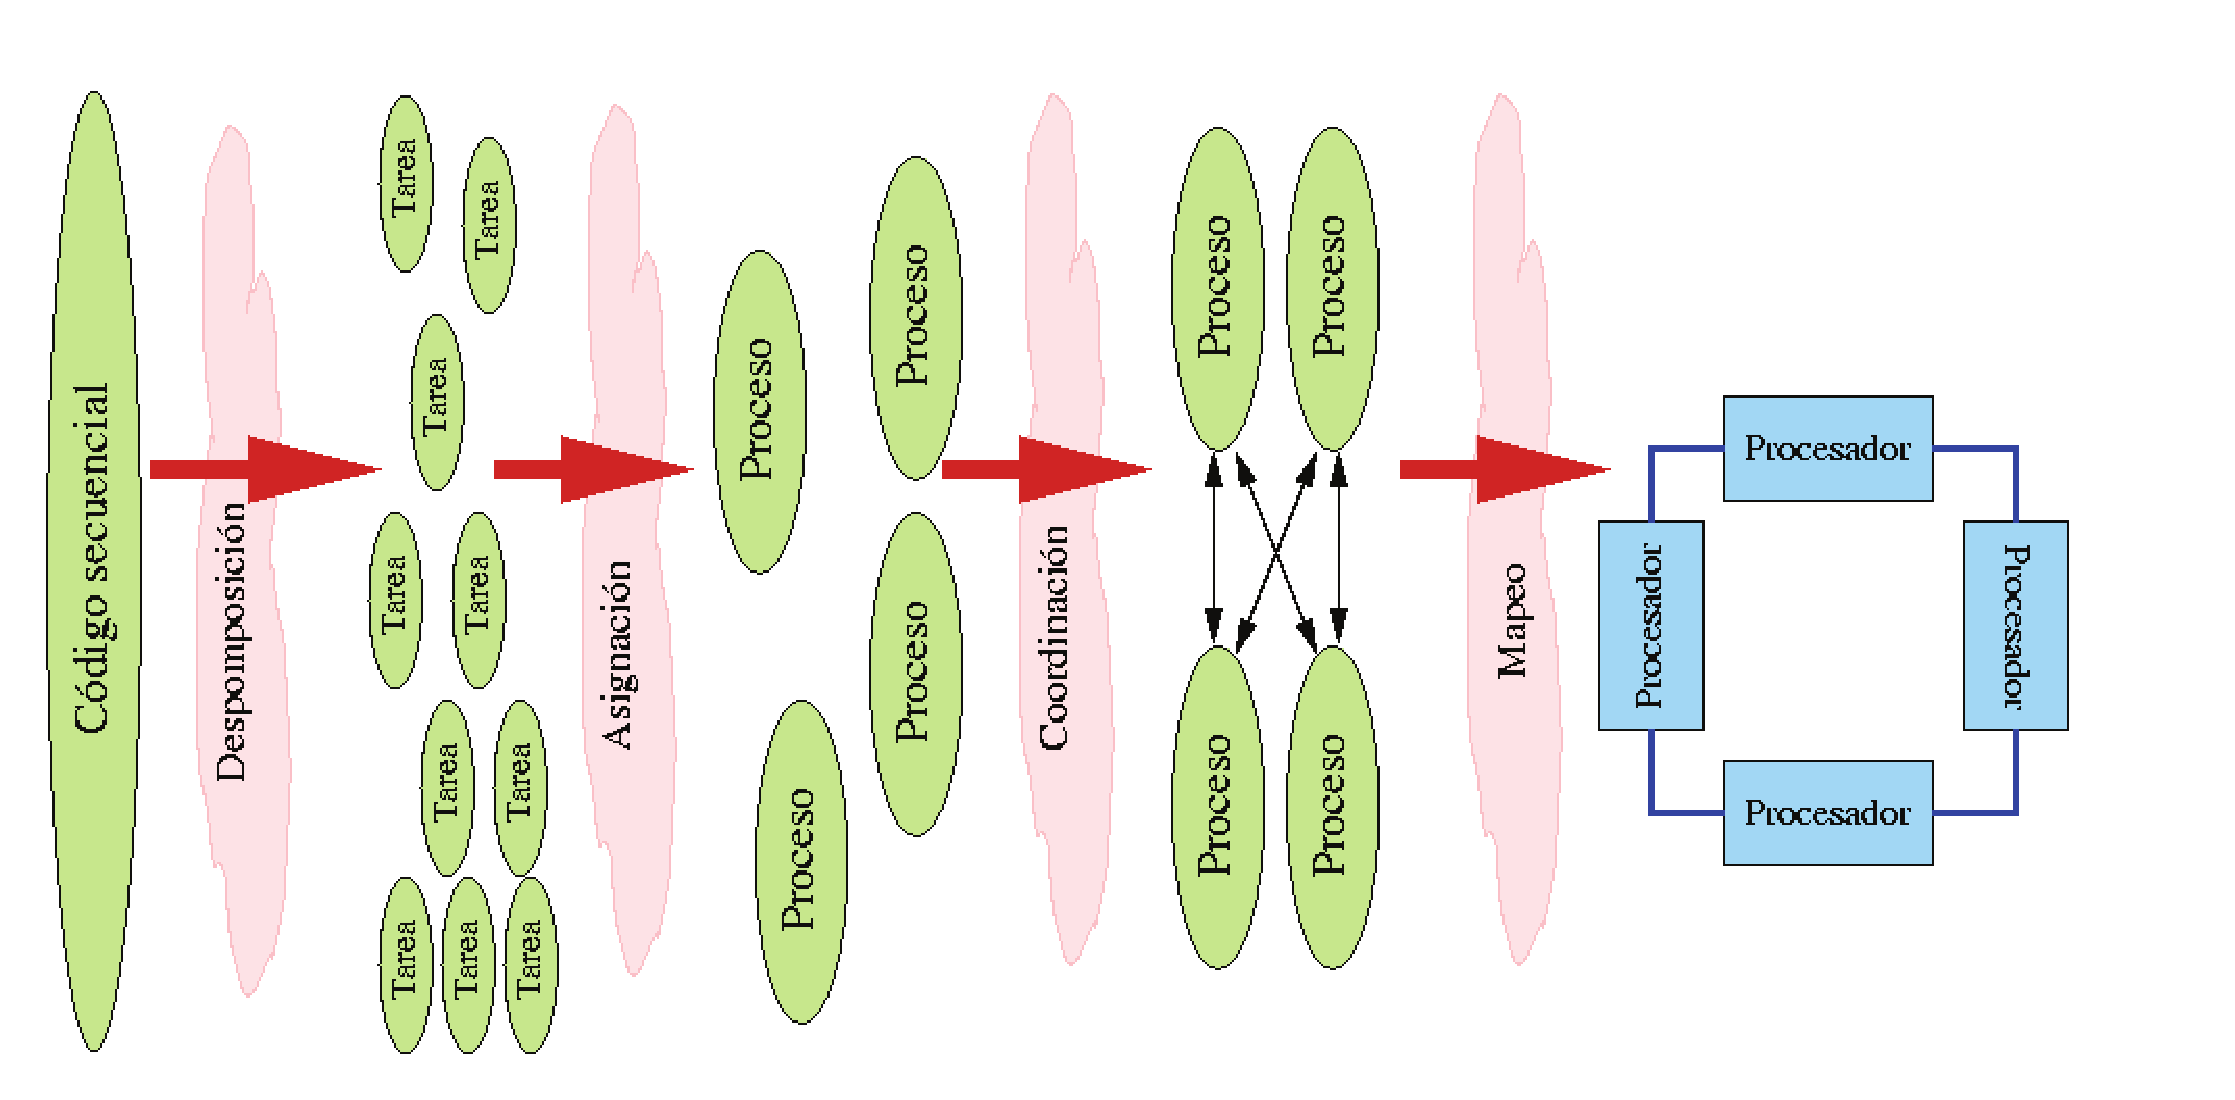
\includegraphics[width=15cm]{figuras/figura01.eps}}
\caption{Esta é a figura de tal e cal.}
\label{enlace1}
\end{figure}

\begin{table}
\begin{center}
\begin{tabular}{|l||r|c|} \hline
Izquierda & Derecha & Centrado  \\ \hline\hline
ll & r & cccc \\ \hline
llll & rrr & c \\ \hline
\end{tabular}
\caption{Esta é a táboa de tal e cal.}
\label{enlace2}
\end{center}
\end{table}

\section{Exemplos de referencias á bibliografía}
Este é un exemplo de referencia a un documento descargado da web \cite{cuda}. E este é un exemplo de referencia a unha páxina da wikipedia \cite{cdma}. Agora un libro \cite{gonzalez} e agora unha referencia a un artigo dunha revista \cite{patricia}. Tamén se poden pór varias referencias á vez \cite{cuda,gonzalez}.

\section{Exemplos de enumeracións}

Con puntos:

\begin{itemize}
\item Un.
\item Dous.
\item Tres.
\end{itemize}

Con números:

\begin{enumerate}
\item Catro.
\item Cinco.
\item Seis.
\end{enumerate}

Exemplo de texto verbatim:

\begin{verbatim}
O texto        verbatim 
     se visualiza tal
            como se escribe
\end{verbatim}

Exemplo de código C:

\lstset{language=C}

\begin{lstlisting}
#include <math.h>
main()
{  int i, j, a[10];
   for(i=0;i<=10;i++) a[i]=i; // comentario 1
   if(a[1]==0) j=1; /* comentario 2 */
   else j=2;
}
\end{lstlisting}

Exemplo de código Java:

\lstset{language=java}

\begin{lstlisting}
class HelloWorldApp {
    public static void main(String[] args) {
        System.out.println("Hello World!"); // Display the string.
    }
}
\end{lstlisting}


